%\section{experience-based control strategy}
\section{off-line work}

%\begin{figure}[H]
%	\centering
%	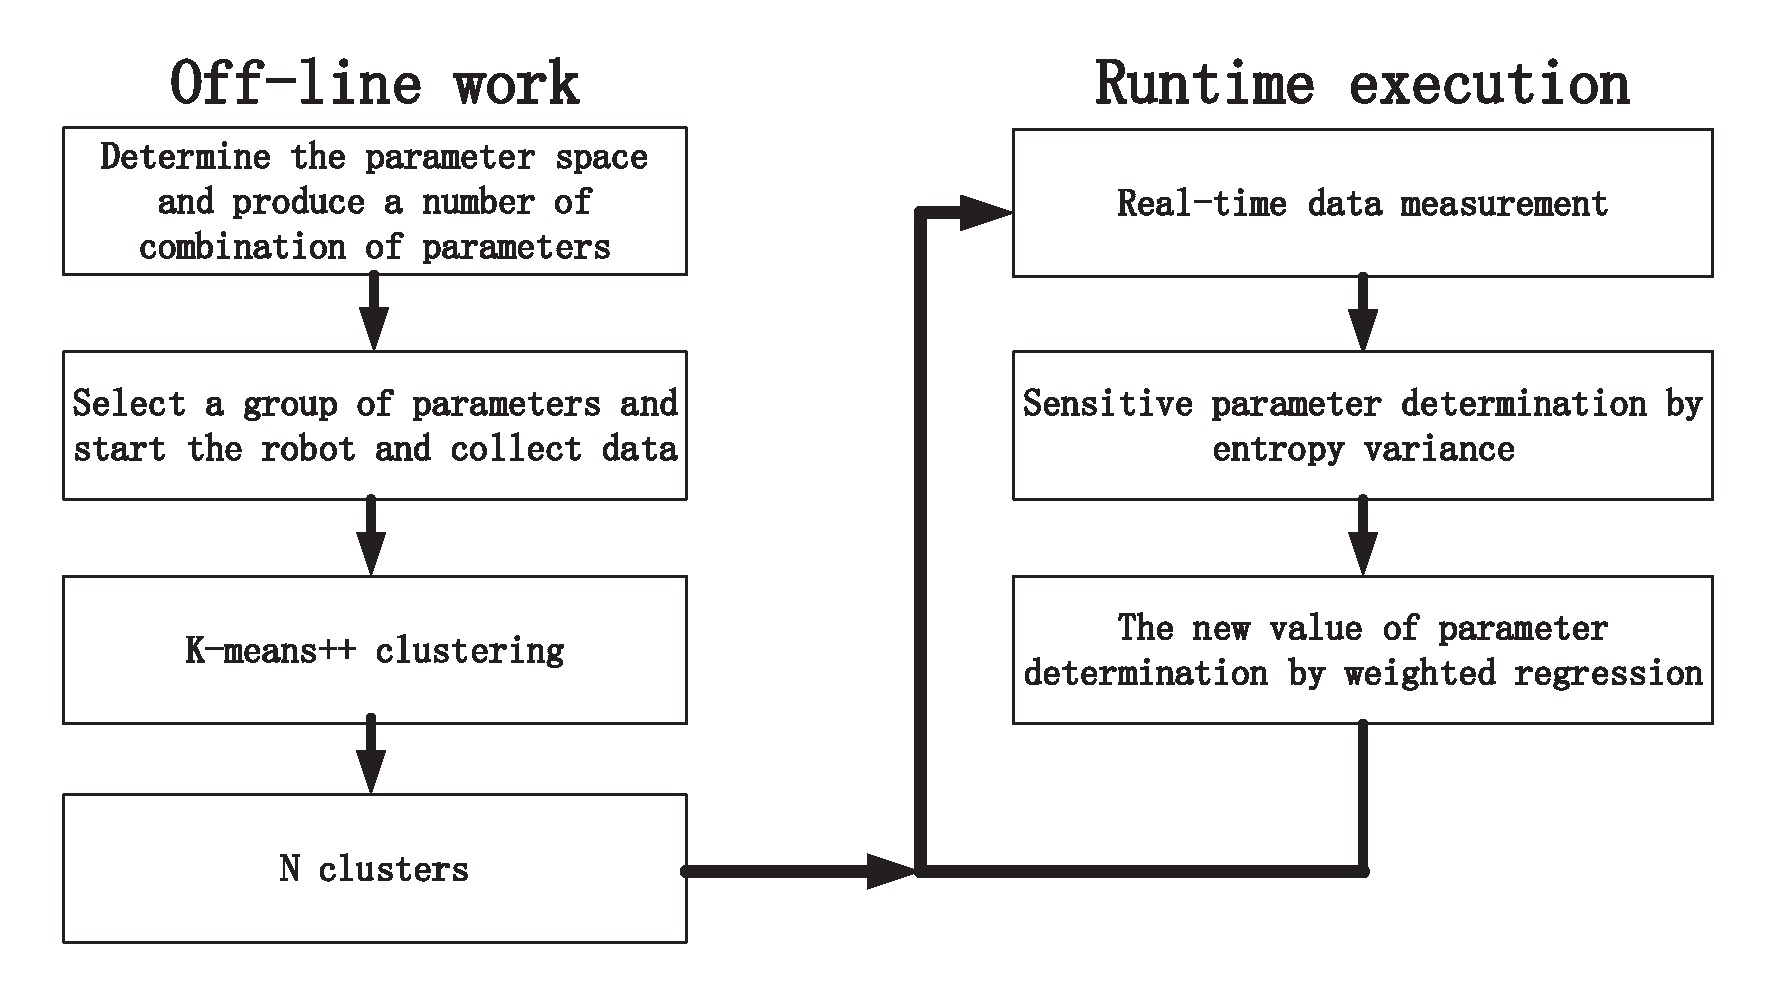
\includegraphics[width=.8\linewidth]{fig/mainwork/stepMap}
%	\caption{The overall experimental flow chart}
%	\figlabel{fig:stepMap}
%\end{figure}

In the preprocessing work, we let the robot move along 25\,cm and 35\,cm poles for a large number of times and we collect and store the data listed in the form like Table \ref{dataTable}.
%\begin{figure}[H]
%	\centering
%	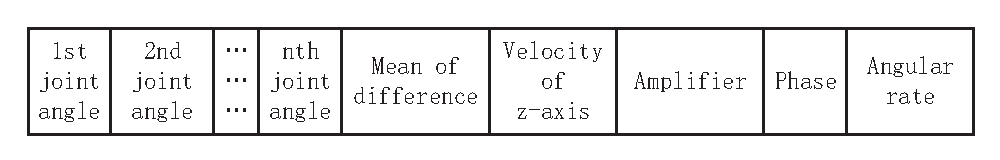
\includegraphics[width=\linewidth]{fig/mainwork/data}
%	\caption{The structure of the data storage}
%	\figlabel{fig:data}
%\end{figure}
\begin{table}[h]
    \begin{center}
        \caption{recorded value during training}
        \label{dataTable}
        \begin{tabular}{cl cl} 
            \toprule
            \multicolumn{1}{m{3cm}}{\centering Symbol}
            &\multicolumn{1}{m{4cm}}
              {\centering Definition}\\
            \midrule
			\multirow{2}{*}{$\theta_{m,i}$} & The joint angle of the $i_{th}$ joint which is\\& measured \\
			\multirow{2}{*}{$M$} & \multirow{2}{*}{Mean of the measured joint angles} \\
			\multirow{2}{*}{$\upsilon_{z}$} & \multirow{2}{*}{The Z-axis velocity} \\\\	\hline
			\multirow{2}{*}{$A$} & \multirow{2}{*}{The value of amplitude} \\
			\multirow{2}{*}{$\omega$} & \multirow{2}{*}{The value of angular rate} \\
			\multirow{2}{*}{$\varepsilon$} & \multirow{2}{*}{The value of phase} \\\\
            \bottomrule
        \end{tabular}
    \end{center}
\end{table}

We define $M$ as $\frac{\sum_{i=1}^{n}\theta_{m,i}}{n} $ where n is the number of joints. $\theta_{m}=\begin{bmatrix}
\theta_{m,1} & \theta_{m,2} & \cdots & \theta_{m,n}
\end{bmatrix}$ is the joint angles which are measured. The control vector is shown as
$\begin{bmatrix}
A& \omega&\varepsilon
\end{bmatrix}$
where $A$ is the amplitude, $\omega$ is the angular rate, and the $\varepsilon$ is the phase. All of them are applied in Eq.\ref{basicRoll}.

After collecting movement data of a snake-liked robot, we combine the training data obtained in different environment and then cluster the data in order to optimize real-time calculation.

%\subsection{Implementation of Clustering by $k-means++$}
In this research, collected data in preprocessing is a large-scale data set. As k-means++ algorithm has high efficiency and scalability for a large-scale data set, we adopt $kmeans++$ for clustering. We classify training set into $N$ clusters. The clustering process is divided into the following steps:
\begin{itemize}
	\item Step 1: Decide the value of $N$ by Eq.\ref{clu_var}.
	\begin{eqnarray}\label{clu_var}
		N=arg\min \limits_{N_{k}}{\frac{\sum _{N_{k}}(S_{i}-E)^{2}}{N_{k}}}
	\end{eqnarray}
	where $E = \frac{\sum _{N}(S_{i})}{N}$ and $i\in [1,N]$.
	\item Step 2: perform k-means++ as \textbf{Algorithm \ref{kmeans}} shows. K-means++ is an improvement on the k-means algorithm. By function INITIALIZE, we can obtain $N$ initial cluster centers. And then, we iterate function UPDATE to update the cluster centers and the clusters until the cluster centers do not change any more.
%	\item Step 2: Randomly select a point in the training set as the first cluster center.
%	\item Step 3: For the $k_{th}$ center, select the point which has the largest  distance to the $(k-1)$ centers in the current training set
	%prework step2
%	\begin{eqnarray}\label{clu_step2}
%	\left\{
%	\begin{array}{lr}
%	F_{c}\left ( P^{\left (  i\right )} \right ) = \sum_{j=1}^{k-1}\left \| X^{\left ( j-1 \right )}-P^{\left (  i\right )} \right \|_{2}\\
%	k = $arg$\max \limits_{i}{(F_{C}(P^{(i)}))}
%	\end{array}
%	\right.
%	\end{eqnarray}
%	\begin{figure}[H]
%		\centering
%		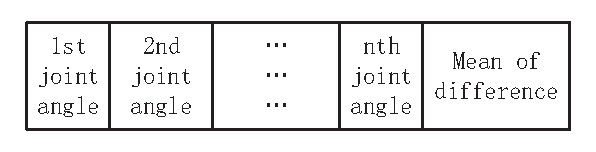
\includegraphics[height=0.5in]{fig/mainwork/data2}
%		\caption{Data vector used in clustering and regression}
%		\figlabel{fig:data2}
%	\end{figure}
%	$P^{(i)}$ is $\begin{bmatrix}
%	\theta_{m} & M
%	\end{bmatrix}$. $X^{(j)}$ is the $j_{th}$ cluster center. $S^{(P)}$ is the  training set. For the initial cluster center $X^{(k)}$, we have $X^{(k)}\in S^{(P)}$ and $X^{(k)}$ is the vector $P^{(i)}$ which corresponds to the result of Eq.\ref{clu_step2}. 
%	\item Step 4: Repeat Step 1 and Step 2 until $N_{k}$ cluster centers have been confirmed.
%	\item Step 5: After confirming $N_{k}$ cluster center, we categorize every vector in training set based on Eq.\ref{clu_step4}.
	%prework step4
%	\begin{eqnarray}\label{clu_step4}
%	C^{(i)} = arg\min \limits_{k}{(||P^{(i)}-X^{(k)}||_{2})}
%	\end{eqnarray}
%	In this equation, $C^{(i)}$ is the flag of category which the vector $P^{(i)}$ belongs to.
%	\item Step 6: Refresh the cluster centers according to clustering result by the Eq.\ref{clu_step5}
	%prework step5
%	\begin{eqnarray}\label{clu_step5}
%	X^{(k)}=\frac{\sum_{i}\{C^{(i)}=k)\}P^{(i)}}{\sum_{i}\{C^{(i)}=k\}}
%	\end{eqnarray}
%	\item Step 7: iterate Step 4 and 5 until the cluster centers change within a predefined tolerance range.
\end{itemize}

\begin{algorithm}
    \caption{k-means++}
    \label{kmeans}
    \begin{algorithmic}[1] 
       \Require Training set $\bm{P}$, The number of clusters $N$
       \Ensure Set of cluster centers $\bm{X}$
       \Function {Initialize}{$\bm{P}, N$}
           \State $\bm{X} \gets sample \ a \ point \ randomly \ from \ \bm{P}$
           \While{$\vert \bm{X} \vert<N$}
               \For{$i = 1 \to \vert \bm{P} \vert$}
                   \State $I \gets arg\min \limits_{i}\left({\sum_{j=1}^{\vert \bm{X} \vert} {\Vert X_j - P_i \Vert}^2  }\right)$
                   \State $\bm{X} \gets \bm{X} \cup \left\{ P_I \right\}$
                   \State $\bm{P} \gets \bm{P} - P_I$
               \EndFor
           \EndWhile
           \State \Return{$\bm{X}$}
       \EndFunction
       \State
       \Function{Update}{$\bm{P}, \bm{X}$}
           \While{$\textbf{X}$ does not change any more}
               \For{$i = 1 \to \vert \bm{P} \vert$}
      \State $C_i \gets arg\min \limits_{k}{\left( {\Vert P_i - X_k\Vert} ^2\right)}$
               \EndFor
               \For{$k = 1 \to \vert \bm{X} \vert$}
      \State $X_k \gets \frac{\sum_{i}{\left\{C_i=k\right\}P_i}}{\sum_{i}{\left\{C_i=k\right\}}}$
               \EndFor
           \EndWhile
           \State \Return{$\bm{X}$}
       \EndFunction
\end{algorithmic}
\end{algorithm}

With $Kmeans++$, the collected data can be divided into $N$ clusters. After finishing the clustering, the result is stored in two parts:

\begin{enumerate}
	\item The cluster centers $\textbf{X}$.
	\item The member $P_{i},i \in [1,\vert \bm{P} \vert]$ of the cluster center $X_{k},k \in [1,N]$
\end{enumerate}

\section{runtime}
In robot's running time, we get the real-time data periodically and then we do the following steps. Firstly, we categorize the real-time data based on the clustering result in off-line work. And then we select the most sensitive gait parameter according to the entropy variance. At last, we use the idea of weighted regression to modify the selected gait parameter and keep the other gait parameters unchanged.
\subsection{Parameter selection by entropy variance}

%classification
\subsubsection{Real-time data categorization}

Every time we get the real-time data, we relegate it to the certain cluster by Eq.\ref{cluster}.
\begin{eqnarray}\label{cluster}
C=arg\min \limits_{k}{(||X_{k}-P_{t}||_{2})} \, ,&X_{C}\in \bm{X}
\end{eqnarray}

$\bm{X}$ is the cluster center set(\textbf{Algorithm \ref{kmeans}}). $X_{C}$ is the closet center to the real-time data vector $P_t$. And $X_{k}$ is the $k_{th}$ cluster center of the cluster center set $\bm{X}$ . With $Euclidian \; Distance \; Formula$, we make a prediction on the similarity between two data vectors.

\subsubsection{The selection of the preponderant data}

After categorization of real-time data, we select those preponderant vectors whose Z-axis velocity are bigger than current (Eq.\ref{preponderant}).
%find out preponderant
\begin{eqnarray}\label{preponderant}
\bm{P_{\upsilon}}=\{P_{i} | \upsilon_{z,i}\geq \upsilon_{z,P_{t}} \; , \; P_{i}\in \bm{P_{C}}\}
\end{eqnarray}

$\bm{P_{C}}$ is all the data vectors which belong to the cluster with the  center $X_{C}$. $\upsilon_{z,i}$ is the vertical velocity component of the data vector $P_{i}$ and $\upsilon_{z,P_{t}}$ is the vertical velocity component of the real-time data vector. $\bm{P_{\upsilon}}$ is the set of all the preponderant vectors for regression.

\subsubsection{The selection of the sensitive parameter}

We adopt entropy variance as the reference to select the parameter which should be modified. The steps of selecting the sensitive parameter are as follows.

\begin{itemize}
	\item Step 1: We take the preprocessing operation to discrete the preponderant data (Eq.\ref{quantification}).
	%quantification
	\begin{eqnarray}\label{quantification}
	\upsilon_{new,i}=\left\{
	\begin{array}{lr}
	\left \lfloor \frac{\upsilon_{z,i}}{L_{D}} \right \rfloor&\upsilon_{z,i}> 0\\
	\\
	\left \lceil \frac{\upsilon_{z,i}-L_{D}}{L_{D}} \right \rceil&\upsilon_{z,i}\leq 0
	\end{array}
	\right.
	\end{eqnarray}
	
	In Eq.\ref{quantification}, $L_{D}$ is the adjustable step length for discretization. We eventually get the velocity discrete sequence:
	\begin{eqnarray}\label{newMember}
	V_{new}=\begin{bmatrix}
	\upsilon_{new,1} & \upsilon_{new,2} & \upsilon_{new,3} & \upsilon_{new,4} & \cdots & \cdots
	\end{bmatrix}
	\end{eqnarray}
	
	\item Step 2: There are a variety of possible values for each gait parameter. Thus, in order to record all the possible values, we make a set $S_{i,j}$ with the gait parameter $i$'s value is its $j_{th}$ possible value. And the value of $i$ is from 0 to 2 representing $A$, $\omega$ and $\varepsilon$ respectively. We calculate the entropy about the vertical velocity when the gait parameter $i$'s value is its $j_{th}$ possible value by Eq.\ref{entropy} as well as the entropy variance of the gait parameter $i$ by Eq.\ref{var_entropy}. In Eq.\ref{entropy}, $p(\upsilon_{new,k})$ is the appearance rate of the $V_{i,j}$ in $S_{i,j}$. In Eq.\ref{var_entropy}, $E_{i,j}$ is the mean of velocity when the gait parameter $i$'s value is its $j_{th}$ possible value. And $N_{i}$ is the number of possible values of the gait parameter $i$.
	%entropy
	\begin{eqnarray}\label{entropy}
	H(S_{i,j})=-\sum _{\upsilon_{new,k}\in V_{new}}p(\upsilon_{new,k})log_{2}p(\upsilon_{new,k})
	\end{eqnarray}
	
	%entropy variance
	\begin{eqnarray}\label{var_entropy}
	Var_{i}=\frac{\sum _{N_{i}}(H(S_{i,j})-E_{i,j})^{2}}{N_{i}}
	\end{eqnarray}
	
	\item Step 3: We normalize the entropy variance (Eq.\ref{normalize}) and randomly select the sensitive gait parameters by Roulette wheel selection algorithm. %(\figref{fig:Roulette}) to avoid the selection getting stuck in the high probability event.
	%normalize entropy variance
	\begin{eqnarray}\label{normalize}
	R_{Var_{i}}=\frac{Var_{i}}{\sum Var_{i}}
	\end{eqnarray}
	
	%\begin{figure}[H]
	%	\centering
	%	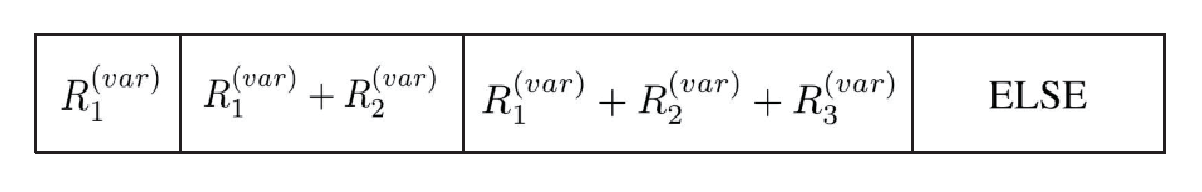
\includegraphics[width=\linewidth]{fig/mainwork/Roulette}
	%	\caption{Sensitive parameter selection by roulette method}
	%	\figlabel{fig:Roulette}
	%\end{figure}
\end{itemize}

After the calculation of gait parameters' entropy variance. the sensitive parameter will be found. And then the selected parameter's value will be modified by regression.


\subsection{Assignment to the value of the selected parameter}

In this research, we take weighted regression to get the value of the sensitive gait parameter and use the gradient descent method to solve the weighted least squares problem in fitting regression function.

\begin{itemize}
	\item Step 1: List the fitting prediction function(Eq.\ref{fitfunction})
	%fitting and estimation function
	\begin{eqnarray}\label{fitfunction}
	F_{w}(P_{t})=W^{T}P_{t}\,,&W=\begin{bmatrix}w_{1}\\ w_{2}\\ \vdots \\ w_{m}\end{bmatrix}
	\end{eqnarray}
	
	In Eq.\ref{fitfunction}, $W$ is the coefficient sequence of the fitting equation and $m$ is the number of coefficients where $P_{t}$ is the real-time collected data vector. Then we can get the error function(Eq.\ref{estimate}) which takes the square of error as the estimation with $n$ being the number of data of $\bm{P_{\upsilon}}$ and $\bm{Q}$ being the set consisting of the value of selected parameter in $P_{i}$.
	%Square sum as an estimation
	\begin{eqnarray}\label{estimate}
		D(W)=\frac{1}{2n}(F_{w}(\bm{P_{\upsilon}})^{T}-\bm{Q})^{T}(F_{w}(\bm{P_{\upsilon}})^{T}-\bm{Q})
	\end{eqnarray}
	\begin{eqnarray}
		\bm{P_{\upsilon}}=\begin{bmatrix}P_{\upsilon,1}&P_{\upsilon,2}  &\cdots  &P_{\upsilon,n} \end{bmatrix}
	\end{eqnarray}
	\begin{eqnarray}
		\bm{Q}=\begin{bmatrix}Q_{\upsilon,1}& Q_{\upsilon,2}& \cdots & Q_{\upsilon,n}\end{bmatrix}^{T}
	\end{eqnarray}
	
	To get the best-fit coefficient sequence $W$ by the minimum $D(w)$, according to gradient descent method, we turn the Eq.\ref{estimate} into Eq.\ref{Gradde}.
	%Gradient descent
	\begin{eqnarray}\label{Gradde}
	\nabla_{w}D=\frac{1}{n}\bm{P_{\upsilon}}(F_{w}(\bm{P_{\upsilon}})^{T}-\bm{Q})
	\end{eqnarray}
	
	\item Step 2: Perform the weighted operation on preponderant data vector to ensure the estimate result of fitting is good (Eq.\ref{WeiGradde}).
	%weighted gradient
	\begin{eqnarray}
	\nabla_{w}D=\frac{1}{n}\bm{P_{\upsilon}}M(F_{w}(\bm{P_{\upsilon}})^{T}-\bm{Q})
	\end{eqnarray}
	\begin{eqnarray}\label{WeiGradde}
	M=\begin{bmatrix}
	\frac{\upsilon_{z,1}}{L_{s}}&0&\cdots&0\\
	0&\frac{\upsilon_{z,2}}{L_{s}}&\ddots&0\\
	\vdots&\ddots&\ddots&0\\
	0&\cdots&0&\frac{\upsilon_{z,3}}{L_{s}}
	\end{bmatrix}
	\end{eqnarray}
	In Eq.\ref{WeiGradde}, $L_s$ is the learning step and $M$ is the learning rate matrix.
	
	\item Step 3: Fit the coefficient vector by Eq.\ref{fit}.
	%fitting the parameters
	\begin{eqnarray}\label{fit}
	W=W-\nabla_{w}D
	\end{eqnarray}
	In this way, the coefficient sequence $W$ is updated.
	
	\item Step 4: Iterate the steps above until we acquire the best-fit coefficient. The value of $W$ is stable finally.
\end{itemize}

When the iteration is stopped, the best-fit coefficient $W_{best}$ will be obtained. By applying $W_{best}$ to Eq.\ref{result}, we can get the regression value of the sensitive parameter. This value will be used in the robot control. It is worth noting that we only modify the sensitive parameter and others remain the same value.
%compensation result
\begin{eqnarray}\label{result}
Q_{t} = F_{w}(P_{t})=W^{T}P_{t}
\end{eqnarray}